
\فصل{مفاهیم اولیه}

در این قسمت مفاهیم مورد استفاده در پایان نامه و همچنین چند اصطلاح رایج در مبحث آزمون نرم‌افزار نوشته شده است
\قسمت{مفاهیم مربوط به میکروسرویس}
\زیرقسمت{میکروسرویس} 
میکروسرویس یک فراروند\پاورقی{Process} منسجم و مستقل است که از طریق پیام‌ در تعامل است. از دیدگاه فنی، میکروسرویس‌ها باید مولفه‌های مستقلی باشند که به صورت مفهومی‌به صورت مجزا مستقر شده و مجهز به ابزارهای اختصاصی ماندگاری حافظه (مانند پایگاه‌های داده) باشند. از آن‌جایی که تمام اجزای یک معماری میکروسرویس، میکروسرویس هستند، رفتار متمایزکننده‌ی آن از ترکیب و تعامل اجزای آن از طریق پیام‌ها ناشی می‌شود. تعاملات بین میکروسرویس‌ها اغلب از طریق مکانیسم‌های سبک، مانند API های منابع از نوع HTTP برقرار می‌شود\مرجع{fowlermsa2014} \مرجع{dragoni2017}. 


\زیرقسمت{میکروسرویس‌ها (معماری میکروسرویس)} 
سبک معماری میکروسرویس\مرجع{fowlermsa2014} رویکردی برای توسعه یک برنامه کاربردی واحد به عنوان مجموعه ای از سرویس‌های کوچک است که هر کدام در فرآروند خاص خود اجرا می‌شوند. برای مثالی از معماری میکروسرویس، فرض می‌کنیم که می‌خواهیم عملکردی ارائه دهیم که نمودار یک تابع را رسم کند. وجود دو میکروسرویس را فرض می‌کنیم: ماشین حساب و نمایشگر. اولین مورد، میکروسرویس ماشین حساب است و دومی‌تصاویر را رنده می‌کند و نمایش می‌دهد. برای تحقق هدفمان، می‌توانیم یک میکروسرویس جدید به نام "رسم‌کننده\پاورقی{Plotter}" معرفی کنیم که ماشین حساب را برای محاسبه شکل نمودار تنظیم می‌کند\پاورقی{Orchestrate} و نمایشگر را برای ارائه شکل محاسبه‌شده فراخوانی می‌کند. در شکل ~\رجوع{شکل:معماری میکروسرویس برای یک برنامه‌ی ماشین حساب}، تصویری از معماری میکروسرویس برنامه‌ی ماشین حساب ذکر‌شده را نمایش داده‌ایم.
\شروع{شکل}[t]
\centerimg{calculator-microservices}{14cm}
\vspace{0.5em}
\شرح{معماری میکروسرویس برای یک برنامه‌ی ماشین حساب\مرجع{dragoni2017}}
\برچسب{شکل:معماری میکروسرویس برای یک برنامه‌ی ماشین حساب}
\پایان{شکل}
توسعه‌دهندگان معماری فوق قادرند به طور جداگانه بر روی اجرای عملکردهای میکروسرویس اصلی، یعنی ماشین حساب و نمایش‌دهنده\پاورقی{Displayer} تمرکز کنند. 
در نهایت، آن‌ها می‌توانند رفتار برنامه‌ی توزیع شده را با رسم‌کننده پیاده‌سازی کنند که در مرحله‌ی 1 تابع کاربر را می‌گیرد، در گام 2 با ماشین حساب تعامل می‌کند تا یک نمایش نمادین از نمودار تابع را محاسبه کند، و در نهایت در گام 3 از نمایش‌دهنده درخواست می‌کند تا نتیجه را به کاربر نشان دهد. 
در مرحله‌‌ی پایانی 4. برای نشان دادن اینکه چگونه رویکرد میکروسرویس با ساخت بر روی معماری‌های میکروسرویسی که از قبل موجود هستند، مقیاس\پاورقی{Scale} می‌شود؛ 
در شکل ~\رجوع{شکل:معماری میکروسرویس برای یک برنامه‌ی ماشین حساب} ماشین حساب به ‌گونه‌ای طراحی شده‌ است که دو میکروسرویس اضافی (به رنگ خاکستری) را که توابع ابتدایی و ویژه ریاضی را اجرا می‌کنند، نیز تنظیم کند. 

سبک معماری میکروسرویس هیچ انگاره\پاورقی{paradigm}ی برنامه نویسی خاصی را مورد حمایت قرار نمی‌دهد یا از هیچ انگاره‌ای منع نمی‌کند؛ بلکه یک دستورالعمل است برای شکستن اجزای یک برنامه کاربردی توزیع شده به موجودیت‌های مستقل که هر یک به یکی از نگرانی‌های آن برنامه می‌پردازد. این بدان معنی است که یک میکروسرویس، به شرطی که عملکردهای خود را از طریق ارسال پیام ارائه دهد، می‌تواند در داخل برنامه با هر زبانی پیاده سازی شود\مرجع{fowlermsa2014}.
میکروسرویس‌ها ممکن است برای ارائه عملکردهای پیچیده‎تر و دقیق‎تر همکاری کنند. دو رویکرد برای ایجاد این همکاری وجود دارد - سبک ارکستراسیون\پاورقی{Orchesteration}\مرجع{mazzara2005} و سبک موزون\پاورقی{Choreography}\مرجع{peltz2003}. ارکستراسیون نیاز به یک رهبر دارد. یک سرویس مرکزی که درخواست‌ها را به سرویس‌های دیگر ارسال می‌کند و با دریافت پاسخ‌ها بر فرآیند نظارت می‌کند. از سوی دیگر، سبک موزون هیچ مرکزیتی ندارد و از رویدادها و مکانیسم‌های انتشار\پاورقی{Publish}/اشتراک\پاورقی{Subscribe} برای ایجاد همکاری استفاده می‌کند. این دو مفهوم برای میکروسرویس‌ها جدید نیستند، بلکه از دنیای معماری بر محوریت سرویس به ارث رسیده‌اند.
قبل از ظهور میکروسرویس‌ها و به طور خاص در آغاز ظهور معماری خدمت‌گرا، به دلیل سادگی استفاده و راه‌حل‌های با هزینه‌ی کمتر برای مدیریت پیچیدگی، عموماً ارکستراسیون محبوب‌تر بود و به طور گسترده‌تر استفاده می‌شد. با این حال، ارکستراسیون به وضوح منجر به جفت‌شدگی\پاورقی{Coupling} سرویس‌ها و توزیع نابرابر مسئولیت‌ها می‌شود، بنابراین برخی از سرویس‌ها نقش متمرکزتری نسبت به سایرین پیدا می‌کنند. فرهنگ تمرکززدایی و درجات بالای استقلال در میکروسرویس‌ها اتفاقا نشان‌دهنده‌ی سناریوی کاربردی ذاتی برای استفاده از سبک موزون برای دستیابی به همکاری است\مرجع{dragoni2017}.

\قسمت{یاول}
بر اساس تجزیه و تحلیل دقیق سیستم‌های مدیریت گردش کار موجود و زبان‌های گردش کار، یک زبان گردش کار جدید به نام یاول (یک زبان دیگر گردش کار) توسط ون‌درآلست\پاورقی{Wil van der Aalst} (استاد دانشگاه فناوری آیندهوون، هلند) و ترهافستید\پاورقی{Arthur ter Hofstede} (استاد دانشگاه صنعتی کوئینزلند، استرالیا) در سال 2002 ایجاد شد. این زبان از یک سو بر شبکه‌های پتری، که یک نظریه همزمانی تثبیت شده با یک نمایش گرافیکی است، و از سوی دیگر بر روی الگوهای گردش کار معروف استوار است. الگوهای گردش کار یک معیار عمومی‌ پذیرفته شده‌ برای مناسب بودن یک زبان توصیف فرآیند است. شبکه‌های پتری\زیرنویس{Petri Nets : یک زبان مدل‌سازی ریاضی برای توصیف سیستم‍های توزیع‌شده.} می‌توانند تعداد کمی از الگوهای کنترل جریان شناسایی شده را جذب کنند، اما آنها از الگوهای چندگانه، الگوهای لغو و پیوند از نوع "یا"ی  تعمیم‌یافته پشتیبانی نمی‌کنند. بنابراین یاول شبکه‌های پتری را با ساختارهای اختصاصی برای پشتیبانی این الگوها گسترش می‌دهد\مرجع{yawlbook}.

یک مدل یاول از مجموعه ای از شبکه‌های یاول به شکل یک ساختار گراف ریشه‌دار تشکیل شده است. هر شبکه یاول از یک سری وظایف تشکیل شده است. وظایف و شرایط در شبکه‌های یاول نقشی مشابه انتقال‌ها و مکان‌ها در شبکه‌های پتری ایفا می‌کنند. هر شبکه یاول دارای یک شرط ورودی و یک شرط خروجی منحصر به فرد است، که نقطه شروع و پایان برای یک نمونه فرآروند است.

وظایف در یک شبکه یاول می‌توانند رفتارهای پیوند و انشعاب خاص خودشان را داشته باشند. ساختارهای پیوند و انشعاب پشتیبانی شده عبارتند از پیوند از نوع "و"، پیوند از نوع "یا"ی انحصاری، پیوند از نوع "یا"، انشعاب از نوع "و"، انشعاب از نوع "یا" و انشعاب از نوع "یا"ی انحصاری. عملکرد هر یک از پیوند و انشعاب‌ها در یاول به شرح زیر است:
\شروع{فقرات}
\فقره پیوند از نوع "و" – شاخه‌ای که به دنبال پیوند از نوع "و" است کنترل را زمانی دریافت می‌کند که تمام شاخه‌های ورودی به پیوند از نوع "و" در یک مورد مشخص فعال شده باشند.
\فقره پیوند از نوع "یا" - شاخه ای که پس از پیوند از نوع "یا" قرار می‌گیرد کنترل را در شرایط زیر دریافت می‌کند: زمانی که (1) همه‌ی شاخه‌های ورودی فعال شده باشند یا (2) همه‌ی شاخه‌های ورودی‌ که هنوز فعال نشده‌اند، امکان فعال شدن در زمان آینده را نداشته باشند.
\فقره پیوند از نوع "یا"ی انحصاری - شاخه‌ای که پس از پیوند از نوع "یا"ی اختصاصی قرار می‌گیرد، کنترل را زمانی دریافت می‌کند که یکی از شاخه‌های ورودی به پیوند از نوع "یا"ی انحصاری فعال شده باشد.
در زبان‌های مختلف رویکردهای مختلف معنایی متفاوت (اغلب فقط شهودی) را به این نوع پیوند اختصاص می‌دهند، اگرچه همه‌‌ی آن‌ها، این موضوع مشترک را دارند که همگام‌سازی فقط برای شاخه‌های فعال انجام می‌شود.
به بیان دقیق‌تر در یاول نگاه کلی به معنای پیوند از نوع "یا"، در حضور ویژگی‌های الغا و بدون محدودیت‌های ساختاری، با استفاده از فرمالیسم شبکه بازنشانی است. شبکه‌های بازنشانی شبکه‌های پتری با قوس‌های بازنشانی هستند. یک قوس بازنشانی زمانی که انتقال آن فعال می‌شود، همه توکن‌ها را از یک مکان حذف می‌کند.
\فقره انشعاب از نوع "و" – زمانی که شاخه‌ی ورودی به انشعاب از نوع "و" فعال می‌شود، کنترل به همه شاخه‌های خروجی انشعاب از نوع "و" منتقل می‌شود.
\فقره انشعاب از نوع "یا"– زمانی که شاخه‌ی ورودی به انشعاب از نوع "یا" فعال می‌شود، کنترل به یک یا چند شاخه‌ی خروجی انشعاب از نوع "یا" بر اساس ارزیابی شرایط مرتبط با هر یک از شاخه‌ها منتقل می‌شود.
\فقره انشعاب از نوع "یا"ی انحصاری – زمانی که شاخه ورودی به انشعاب از نوع "یا"ی انحصاری فعال می‌شود، کنترل دقیقاً به یکی از شاخه‌های خروجی انشعاب از نوع "یا"ی انحصاری بر اساس ارزیابی شرایط مرتبط با هر یک از شاخه‌ها منتقل می‌شود.
\پایان {فقرات}

یاول از مفهوم منطقه‌ی لغو پشتیبانی می‌کند، که شامل گروهی از وظایف در یک شبکه یاول است. منطقه‌ی لغو به یک وظیفه‌ی خاص در همان شبکه یاول مرتبط است. در زمان اجرا، زمانی که نمونه‌ای از وظیفه‌ای که منطقه لغو به آن متصل است، اجرا را کامل می‌کند، تمام وظایف موجود در منطقه لغو مرتبط که در حال حاضر برای همان مورد در حال اجرا هستند، لغو می‌شوند.

\زیرقسمت{ساختار ذخیره‌سازی مدل‌ها در زبان یاول}
مدل‌های تولیدشده به زبان یاول در قالب استاندارد XML ذخیره می‌شوند؛ استفاده از فرمت استاندارد XML برای ذخیره مدل‌های یاول، امکان ذخیره و تبادل داده‌ها بین سیستم‌های مختلف را در یک فرمت قابل استفاده و قابل خواندن فراهم می‌کند. با استفاده از فرمت استاندارد، امکان تبادل ساده و راحت مدل‌های یاول بدون توجه به مکان و پلتفرم نرم‌افزاری آن‌ها، بین افراد و تیم‌های مختلف وجود دارد.

\قسمت{الوی}
الوی یک زبان توصیف برای بیان محدودیت‌ها و رفتار ساختاری پیچیده در یک سیستم نرم افزاری است و همچنین یک ابزار مدل سازی ساختاری ساده بر اساس منطق مرتبه اول ارائه می‌دهد\مرجع{alloybook}.

الوی از موفقیت‌ها و محدودیت‌های چک کننده‌ی مدل‌ها الهام گرفته شده است و نوع جدیدی از زبان طراحی و تحلیل ارائه می‌دهد که با سه نوآوری امکان پذیر شده‌ است:
\شروع {فقرات}
\فقره اولین آن‌ها منطق رابطه‌ای است، الوی از این منطق برای توصیف طراحی‌ها و ویژگی‌ها استفاده می‌کند. منطق رابطه‌ای\مرجع{AGUIRRE2019}، کمیت‌کننده\پاورقی{quantifier}‌های منطق مرتبه اول را با عملگرهای نظریه‌ی مجموعه‌ها و حساب رابطه‌ای می‌آمیزد. ایده‌ی مدل‌سازی طرح‌های نرم‌افزاری با مجموعه‌ها و روابط در زبان Z مطرح شده بود\مرجع{z-notation} الوی از بخش زیادی از قدرت Z استفاده کرده است، در حالی که منطق موجود در آن را ساده‌تر می‌کند تا Z را قابل استفاده‌تر کند. در این راستا الوی فقط ساختارهای مرتبه اول را استفاده می‌کند. الوی همچنین تحت تأثیر زبان‌های مدل سازی مانند UML است.

\فقره نوآوری دوم در الوی استفاده از تجزیه و تحلیل دامنه کوچک است. حتی منطق مرتبه اول ساده (بدون عملگرهای رابطه‌ای) تصمیم‌پذیر نیست. این به این معنی است که هیچ الگوریتمی نمی‌تواند وجود داشته باشد که بتواند طراحی نرم افزاری که به طور کامل به زبانی مانند الوی نوشته شده است را تجزیه و تحلیل کند. می‌توان زبان را تصمیم‌پذیر کرد، اما این امر قدرت بیان آن را ناقص می‌کند و باعث می‌شود که نتواند حتی ابتدایی‌ترین ویژگی‌های ساختارها را بیان کند. برای داشتن تجزیه و تحلیل چنین برنامه‌هایی یک راه این است که خودکارسازی تجزیه و تحلیل را حذف کرد و از کاربر برای این کار کمک گرفت. اما این کار مزایای یک ابزار تجزیه و تحلیل را ضایع می‌کند. در این صورت تجزیه و تحلیل دیگر پاداشی برای ساخت یک مدل طراحی نیست، بلکه یک سرمایه گذاری اضافی بزرگ و فراتر از مدل‌سازی است.

یک راه دیگر نیز محدود کردن تحلیل است که پیش از الوی از راه‌های انتزاع و شبیه‌سازی استفاده می‌شد. انتزاع معمولا آنقدر از جزئیات می‌کاست که به ایجاد مثبت نادرست منجر می‌شد که قابل تفسیر هم نبود و شبیه‌سازی نیز آنقدر بخش کوچکی از فضای حالت را پوشش می‌داد که نقص‌های ظریف از تشخیص فرار می‌کردند. اما یاول یک رویکرد جدید ارائه کرد: اجرای تمام آزمون‌های کوچک. طراح، محدوده‌ای را مشخص می‌کند که هر یک از انواع را در توصیف محدود می‌کند. این نوآوری بر پایه‌ی فرضیه دامنه کوچک\مرجع{oetsch2012}\پاورقی{فرضیه‌ای که بیان می‌کند نسبت بالایی از خطاها را می‌توان با آزمایش یک برنامه برای همه ورودی‌های تست در محدوده کوچکی یافت} است، که ادعا می‌کند اکثر خطاها را می‌توان با مثال‌های نقض کوچک مشخص کرد.

\فقره سومین نوآوری الوی در ترجمه‌ی مدل‌ها به یک مساله‌ی صدق‌پذیری است. حتی با محدوده‌های کوچک، فضای حالت یک مدلِ الوی، بسیار بزرگ است. حالت شامل مجموعه ای از متغیرها است که مقادیر آنها، روابط بین انواع هستند. فقط یک رابطه‌ی دودویی در یک محدوده‌ی پنج تایی دارای 5 × 5 = 25 یال ممکن است، و بنابراین می‎تواند
$2 ‌^ {25} $
 مقدار ممکن داشته باشد. یک طرح بسیار کوچک ممکن است دارای پنج رابطه باشد که به
$(2 ^ {25}) ^ 5 $
 حالت ممکن - حدود
$10 ^ {37} $
  حالت می‌شود. حتی با بررسی یک میلیارد مورد در ثانیه، چنین تحلیلی چندین برابر عمر جهان است. بنابراین الوی یک جستجوی صریح انجام نمی‌دهد، بلکه در عوض مسئله‌ی طراحی را به یک مسئله رضایت‌پذیری تبدیل می‌کند که متغیرهای آن روابط نیستند بلکه بیت‌های ساده هستند. با چرخش بیت‌ها به صورت جداگانه، یک حل‌کننده رضایت‌پذیری معمولاً می‌تواند راه‌حلی را بیابد (اگر وجود داشته باشد) یا تنها با بررسی بخش کوچکی از فضا نشان دهد که هیچ راه‌حلی وجود ندارد. ابزار تجزیه و تحلیل الوی اساساً یک کامپایلر برای مساله‌ی رضایت‌پذیری است که به آن اجازه می‌دهد از آخرین پیشرفت‌ها در حل کننده‌های مساله‌ی رضایت‌پذیری بهره‌برداری کند. موفقیت حل کننده‌های مساله‌ی رضایت‌پذیری یک داستان قابل توجه در علم کامپیوتر بوده است - نظریه‌پردازان نشان داده بودند که مساله‌ی رضایت‌پذیری ذاتاً غیر قابل حل است، اما معلوم شد که بیشتر مواردی که در عمل پدیدار می‌شوند، می‌توانند به طور موثر حل شوند. بنابراین مساله‌ی رضایت‌پذیری از یک مسئله‌ی حل‌نشدنی کهن الگو که برای نشان دادن غیرممکن بودن مسائل دیگر استفاده می‌شد، به یک مساله‌ی حل‌شدنی تبدیل شد که سایر مسائل را می‌توان به آن ترجمه کرد. الوی همچنین از روش‌های مختلفی برای کاهش مساله‌ قبل از حل استفاده می‌کند، به ویژه افزودن محدودیت‌های شکست تقارن که حل‌کننده مساله‌ی رضایت‌پذیری را از در نظر گرفتن موارد مشابه با یکدیگر باز ‌می‌دارد\مرجع{jackson2019}.
\پایان {فقرات}

زبان الوی مانند زبان‌های توصیف نرم‌افزار دیگر دارای ابزارهایی برای نظام‌دهی مدل‌ها، ساخت مدل‌های بزرگ‌تر از مدل‌های کوچک‌تر و ساخت مولفه‌ها با قابلیت استفاده‌ی مجدد است، همچنین جزئیاتی در نحو آن وجود دارد تا الوی زبانی قابل استفاده در عمل باشد. 
مدل‌ها در الوی به صورتی مشخص و با نحو الوی توصیف می‌شوند، اجزایی از الوی که در این پایان‌نامه مورد استفاده قرار گرفته‌اند، را در ادامه آورده‌ایم و در انتها نیز در یک مثال از آن‌ها برای توصیف یک نرم‌افزار ساده استفاده کرده‌ایم.
امضا: یک امضا مجموعه ای از اتم‌ها را معرفی می‌کند. امضا
\کد{sig A\{\}}
مجموعه‌ای به نام A را معرفی می‌کند. امضا در واقع چیزی بیش از یک مجموعه است، زیرا می‌تواند شامل اعلام روابط باشد و می‌تواند به طور ضمنی نوع جدیدی را معرفی کند.
یک مجموعه را می‌توان به عنوان زیرمجموعه‌ای دیگر معرفی کرد. از آن جایی که یک امضا در واقع یک مجموعه نیز هست در نتیجه
\کد{sig A1 extensions A \{\} }
مجموعه‌ای به نام A1 را معرفی می‌کند که زیرمجموعه A است. امضای A1 توسعه‌داده‌شده یا زیرامضای امضای A است.

در الوی مفروضات در "حقیقت‌"ها قرار می‎گیرند. مفاهیمی که باید بررسی شوند در اظهارها گفته می‌شوند. محدودیت‌هایی که در زمینه‎های مختلف لازم‌اند. به عنوان مسند تعریف می‌شوند.
با استفاده از یک مثال در زیر نشان می‌دهیم که چگونه می‌توان با استفاده از ابزارها و نحو الوی، یک مدل ساده را به صورت سازگار توصیف کرد.

\شروع{شکل}[t]
\centerimg{traffic-light}{8cm}
\vspace{0.5em}
\شرح{سیستم چراغ راهنمایی{alloybook}}
\برچسب{شکل: سیستم چراغ راهنمایی}
\پایان{شکل}

شکل ~\رجوع{شکل: سیستم چراغ راهنمایی}، یک سیستم چراغ راهنمایی را نشان می‌دهد. در این سیستم می‌خواهیم که در هر تقاطع، در هر حالتی، بعضی از چراغ‌ها قرمز را نشان دهند. برای این سیستم در الوی قطعه توصیف زیر را می‌توان نوشت:
\شروع{شکل}[h]
\raggedright
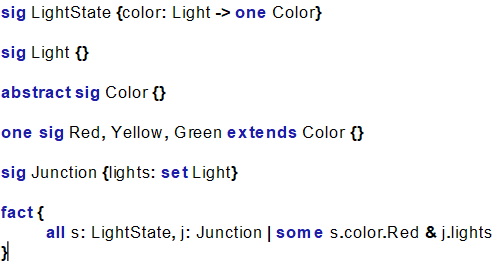
\includegraphics[width=10cm]{traffic-light-specification}
\vspace{0.05em}
\برچسب{شکل:توصیف صوری سیستم چراغ راهنمایی با زبان الوی}
\پایان{شکل}




\زیرقسمت {تحلیل‌گر الوی}
تحلیل‌گر الوی ابزاری است که در واقع توصیفات نوشته شده به زبان الوی را بررسی می‌کند. تحلیلگر مدل را به فرمول صدق‌پذیری برای حل تبدیل می‌کند. این تحلیل که در تحلیل‌گر الوی گنجانده شده است، بر پیشرفت‌های اخیر در فناوری صدق‌پذیری متکی است. تحلیل‌گر الوی محدودیت‌هایی را که باید حل شوند از الوی به محدودیت‌های بولی ترجمه می‌کند، که به یک حل‌کننده‌ی صدق‌پذیری آماده به کار داده می‌شود. همانطور که حل کننده‌های مساله‌ی صدق‌پذیری سریع‌تر می‌شوند، تجزیه و تحلیل الوی نیز سریع‌تر می‌شود و به مسائل بزرگ‌تر می‌رسد. با استفاده از بهترین حل کننده‌های امروزی، تحلیلگر می‌تواند فضاهایی را که چند صد بیت عرض دارند بررسی کند.

تحلیلی که تحلیل‌گر الوی انجام می‌دهد نوعی حل محدودیت است. اما نقطه‌ی قوت تحلیل‌گر الوی در شبیه‌سازی سیستم مدل‌شده با الوی است. شبیه‌سازی شامل یافتن نمونه‌هایی از حالت‌ها یا اجراهایی است که یک ویژگی معین را برآورده می‌کند. همچنین می‌توان با تحلیل‌گر الوی مثال نقض برای حالت‌های خاص تعریف‌شده با الوی یافت. در این جا مقصود از مثال نقض نمونه‌ای است که یک ویژگی معین را نقض می‌کند. این ویژگی معین با اظهارها بیان می‌شوند. جستجوی نمونه‌ها در فضایی انجام می‌شود که ابعاد آن توسط کاربر در یک محدوده مشخص شده است، که یک کران به تعداد اشیاء از هر نوع اختصاص می‌دهد. حتی یک محدوده‌ی کوچک، یک فضای بزرگ را تعریف می‌کند، بنابراین استفاده از تحلیل‌گر الوی اغلب برای یافتن خطاها در فضاهای کوچک مناسب است.



\قسمت {آزمون}
با رشد صنعت نرم‌افزار، آزمون نرم‌افزار نیز به عنوان فعالیتی کلیدی برای تضمین کیفیت پیشرفت کرده است، اگرچه عوامل بسیاری، از جمله، طراحی دقیق و مدیریت فرآیند کامل، بر مهندسی نرم افزار قابل اتکا تأثیر می‌گذارند، اما آزمون، اولین روشی است که صنعت، از آن برای ارزیابی نرم افزار در طول توسعه بهره می‌برد. بیزر\پاورقی{Beizer} هدف از آزمون محصول نرم‌افزاری را بر حسب «سطوح بلوغ فرآیند آزمون» یک سازمان بیان می‌کند، به طوری که این سطوح با اهداف آزمون‌کنندگان از آزمون تعیین می‌شوند\مرجع{beizer1990}.

از آن‌جایی که واژه‌ی "درستی" در محصولات مهندسی واژه‌ای مبهم است و نمی‌توان منظور از درستی محصول را به صورت دقیق بیان کرد. مهندسان نرم‌افزار خردمند به جای جستجوی «درستی»، سعی می‌کنند «رفتار» نرم‌افزار را ارزیابی کنند تا تصمیم بگیرند که آیا این رفتار با در نظر گرفتن تعداد زیادی از عوامل از جمله قابلیت اطمینان، ایمنی، قابلیت نگهداری، امنیت و کارایی قابل قبول است یا خیر. بدیهی است که این بسیار پیچیده‌تر از میل ساده لوحانه برای نشان دادن درستی نرم‌افزار است. مهندسان نرم‌افزار برای مقابله با چنین پیچیدگی طاقت فرسایی از "بالا بردن سطح انتزاع" استفاده می‌کنند.
 
کار توسعه آزمون‌ها را می‌توان به چهار بخش مجزا تقسیم کرد: طراحی آزمون، خودکارسازی آزمون، اجرای آزمون و ارزیابی آزمون.


\شروع{شمارش}
\فقره طراحی آزمون فرآروند طراحی مقادیر ورودی است که به طور موثر نرم‌افزار را آزمایش می‌‌کند. این ریاضیاتی‌ترین و از نظر فنی چالش برانگیزترین بخش آزمون است. که می‌تواند به روش‌های مبتنی بر قاعده یا روش‌های مبتنی بر انسان انجام شود. استفاده از روش‌های مبتنی بر قاعده نیاز به دانش ریاضیات گسسته، برنامه‌نویسی و البته آزمون دارد. در حالی که روش‌های مبتنی بر انسان نیاز به دانش دامنه‌ی کاربرد نرم‌افزار مورد آزمون، واسط‌های کاربری و خود آزمون دارد.

\فقره خودکارسازی آزمون، فرآروند جاسازی مقادیر آزمون در برنامه‌ی اجرا شونده است. جایی که مقادیر آزمون همان خروجی نهایی مرحله‌ی طراحی آزمون است.

\فقره اجرای آزمون فرآروند اجرای آزمون‌ها بر روی نرم‌افزار و ثبت نتایج است. این مرحله، نیاز به دانش ابتدایی نرم‌افزار برای انجام دارد. امروزه بیشتر سازمان‌ها برای رسیدن به خودکارسازی صد در صد آزمون‌ها تلاش می‌کنند، این هدف اجرای آزمون‌ را به طرز قابل ملاحظه‌ای ساده می‌کند.
فرآروند طراحی آزمون مدل‌رانه، آزمون را به یک مجموعه کارهای کوچک تقسیم می‌کند که تولید آزمون را ساده می‌کند. سپس طراحان آزمون کار خود را به صورت جداگانه و فارغ از جزئیات نرم‌افزار یا مصنوعات طراحی، اتوماسیون آزمون و اجرای آزمون در سطح بالاتری از انتزاع پیش می‌برند و با استفاده از ساختارهای مهندسی ریاضیاتی مقادیر آزمون را طراحی می‌کنند. 

\فقره ارزیابی آزمون فرآروند ارزیابی نتایج آزمون و گزارش‌دهی به توسعه‌دهندگان است. انجام این مرحله نیاز به مهارت‌هایی مشابه مهارت‌های مورد نیاز برای طراحی آزمون با روش‌های مبتنی بر انسان دارد. ارزیابی آزمون اغلب با بیان خروجی‌های مورد انتطار در قالب  اظهارها انجام می‌شود\مرجع{testingbook}.
\پایان{شمارش}




\مهم{آزمون مدل-رانه}

در طراحی آزمون مدل-رانه ما آزمون‌های خود را از ساختارهای انتزاعی که بسیار شبیه به مدل‌ها هستند استخراج می‌کنیم. این ساختارهای انتزاعی می‌توانند نمودارهای وضعیت در UML، شبکه‌های پتری، گراف‌ها یا توصیفات صوری باشند. 

طراحی آزمون مدل-رانه به طراحان آزمون اجازه می‌‌دهد «سطح انتزاع خود را بالا ببرند» به طوری که زیر مجموعه‌ی کوچکی از آزمون‌کنندگان، جنبه‌های ریاضی طراحی و توسعه آزمون‌ها را انجام می‌دهند. سپس آزمون‌کنندگان و برنامه‌نویسان دیگر می‌توانند بخش‌های خود که شامل یافتن مقادیر آزمون، خودکار کردن آزمون‌ها، اجرای آزمون‌ها و ارزیابی آن‌ها، می‌شود را انجام ‌دهند. این مشابه طراحی ساختمانی است، جایی که یک مهندس طرحی را ایجاد می‌‌کند که توسط بسیاری از متخصصین و کارگران دنبال می‌شود. 

فرآیند طراحی آزمون مدل-رانه به صراحت از تقسیم کار پشتیبانی می‌‌کند. فرآروند این نوع از طراحی در شکل زیر نشان داده شده است، فعالیت‌های طراحی آزمون را در بالای خط و سایر فعالیت‌های آزمون را در شکل ~\رجوع{شکل: آزمون مدل-رانه}، می‌بینیم.

\شروع{شکل}[t]
\centerimg{model-driven-testing}{14cm}
\vspace{0.5em}
\شرح{آزمون مدل-رانه\مرجع{testingbook}}
\برچسب{شکل: آزمون مدل-رانه}
\پایان{شکل}


\مهم{مدل خطا/شکست}

تفاوتی اساسی بین عمل اشکال‌زدایی و عمل آزمون وجود دارد. در اشکال‌زدایی برای یک شکست موجود به دنبال علت هستیم در حالی که در فرآروند آزمون به دنبال کمینه کردن مخاطره‌ی استفاده از نرم‌افزار هستیم. مسئله اصلی این است که برای یک خطای معین، که در اشکال‌زدایی به ما داده شده‌است، همه ورودی‌ها باعث ایجاد خطا در ایجاد خروجی نادرست (شکست) نمی‌‌شوند. همچنین، ربط دادن یک شکست به خطایی که باعث آن شده است، اغلب بسیار دشوار است. تجزیه و تحلیل این ایده‌ها منجر به مدل خطا/شکست می‌شود که بیان می‌‌کند چهار شرط برای مشاهده‌ی شکست لازم است.

شکل ‍~\رجوع{شکل: مدل خطا/شکست و شرایط RIPR} شرایط را نشان می‌‌دهد. ابتدا، یک آزمون باید به مکان یا مکان‌هایی در برنامه برسد که حاوی خطا (قابل دسترس بودن) هستند. دوما، پس از اجرای برنامه در آن مکان، حالت برنامه باید نادرست باشد (سرایت). سوما، حالت آلوده باید در بقیه مراحل اجرا منتشر شود و باعث شود برخی خروجی‌ها یا وضعیت نهایی برنامه نادرست شوند.(انتشار). در نهایت، آزمون‌کننده باید بخشی از قسمت نادرست حالت نهایی برنامه (قابل آشکار شدن) را مشاهده کند. اگر آزمون‌کننده فقط قسمت‌هایی از حالت نهایی برنامه را ببیند که صحیح هستند، خرابی آشکار نمی‌شود. مدل خطا/شکست در شکل ~\رجوع{شکل: مدل خطا/شکست و شرایط RIPR} مشخص شده است.

\شروع{شکل}[t]
\centerimg{fault-failure-model}{14cm}
\vspace{0.5em}
\شرح{مدل خطا/شکست و شرایط RIPR\مرجع{testingbook}}
\برچسب{شکل: مدل خطا/شکست و شرایط RIPR}
\پایان{شکل}

\مهم{مورد آزمون}

یک مورد آزمون از مقادیر آزمون، مقادیر پیشوند، مقادیر پسوند و نتایج مورد انتظار لازم برای اجرای کامل و ارزیابی نرم افزار تحت آزمایش تشکیل شده است.

\مهم{مجموعه آزمون}

مجموعه آزمون مجموعه ای از موارد آزمون است.

\مهم{نیازمندی آزمون}

یک نیازمندی آزمون عنصر خاصی از یک مصنوع نرم‌افزاری است که یک مورد آزمون باید آن را برآورده کند یا پوشش دهد.



\مهم{معیار پوشش}

تعداد ورودی‌های بالقوه برای اکثر برنامه‌ها به قدری زیاد است که می‌توان عملا آن را بی‌نهایت دانست زیرا که نمی‌توان به صراحت ورودی‌ها را برشمرد. اینجاست که معیارهای پوشش رسمی(یا صوری بهتره) وارد می‌شوند. از آنجایی که نمی‌توانیم با همه‌ی ورودی‌ها برنامه را بیازماییم، از معیارهای پوشش برای تصمیم‌گیری درباره‌ی ورودی‌های آزمون استفاده می‌کنیم. منطق پشت معیارهای پوشش این است که آنها فضای ورودی را برای به حداکثر رساندن تعداد خطاهای یافت‌شده در هر مورد آزمون تقسیم می‌کنند. مزیت دیگر برای استفاده از معیارهای پوشش در عمل این است که آن‌ها قوانین مفیدی را برای زمان توقف فرآروند آزمون ارائه می‌کنند. 

تعریف رسمی معیار پوشش، آن را یک قاعده یا مجموعه قوانینی معرفی می‌کند که الزامات آزمون را بر یک مجموعه آزمون تحمیل می‌کند.
معیار‌های رایج‌ که برخی از آن‌ها مطابق با مدل خطا/شکست تعریف ‌شده‌اند و استفاده می‌شوند عبارتند از پارتیشن‌بندی فضای ورودی که طراحی تست را به روشی مستقل از مدل خطا/شکست انجام می‌دهد زیرا که فقط از فضای ورودی نرم‌افزار تحت آزمون استفاده می‌کند؛ معیارهای پوشش گراف که قابل دسترس بودن را تضمین می‌کند، استفاده از عبارات منطقی برای تولید آزمون که سرایت را تضمین می‌کند و تجزیه و تحلیل جهش که انتشار را تضمین می‌کند.

\مهم{پوشش}

با توجه به مجموعه ای از نیازمندی‌های آزمون \کد{TR} برای یک معیار پوشش \کد{C}، یک مجموعه آزمون \کد{T}، \کد{C} را برآورده می‌کند اگر و تنها اگر برای هر نیازمندی آزمون \کد{tr} در \کد{TR}، حداقل یک آزمون \کد{t} در \کد{T} وجود داشته باشد به طوری که \کد{t} را ارضا کند.

\مهم{معیار‌های پوشش بر اساس منطق}

معیارهای پوشش بر اساس منطق از عبارات منطقی برای تعریف معیارها و طراحی آزمون‌ها استفاده می‌کند. این دسته از معیارها به پیشرفت ما در مدل خطا/شکست کمک می‌کنند و اطمینان حاصل می‌کنند که آزمون‌ها نه تنها به مکان‌های خاصی می‌رسند، بلکه حالت داخلی برنامه نیز متاثر از انتساب ترکیب‌های مختلفی از درستی به عبارات، آلوده می‌شود.
از گزاره‌ها و مسندها برای معرفی انواع معیارهای پوشش استفاده می‌‌شود. فرض کنید \کد{P} مجموعه‌ای از مسندها و \کد{C} مجموعه‌ای از گزاره‌ها در مسندهای \کد{P} باشد. برای هر مسند 
$p \in P$، 
$C_p$ گزاره‌های در \کد{p} باشد به طوری که 
$C_p = \{c| c \in p\}$
مجموعه‌ی \کد{C} اجتماع گزاره‌های موجود در هر یک از مسندها در \کد{P} خواهد بود، به عبارتی 
$C = \cup_{p\in P} C_{p\textasciicircum.}$

\مهم{پوشش گزاره}

برای هر 
$c \in C$
\کد{TR} شامل دو نیازمندی است: اطلاق \کد{c} به "درست" و اطلاق \کد{c} به نادرست. گزاره‌ی
$a \vee b$
 را در نظر بگیرید. گزاره‌های \کد{C} عبارتند از 
 $\set{a, b}$
 چهار ورودی آزمون که ترکیبی از مقادیر منطقی برای گزاره‌ها را برمی‎شمارد در جدول صحت زیر آمده، مشخص است.

\شروع{شکل}[h]
\raggedright
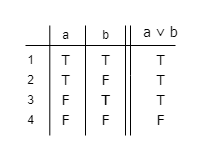
\includegraphics[width=7cm]{cc-coverage}
\vspace{0.1em}
\برچسب{شکل: جدول درستی برای پوشش گزاره}
\پایان{شکل}
مجموعه تست 
$T_{23} = \set{2, 3}$
 پوشش گزاره را برآورده می‌کند.

با توجه به تعاریف بالا می‌توان پوشش‌های زیر را بیان کرد

\مهم{پوشش گزاره‌ی فعال}

برای تعریف پوشش گزاره‌ی فعال ابتدا باید بدانیم گزاره‌ی اصلی یا تعیین‌کننده چیست. با در نظر گرفتن یک گزاره‌ی اصلی 
$c_i$
 در مسند \کد{p}، می‌گوییم که اگر جملات فرعی
$c_j \in p، j \neq i$
 مقادیری داشته باشند، 
 $c_i$
 \کد{p} را تعیین می‌‌کند به طوری که تغییر مقدار صدق 
$c_i$
 ، ارزش \کد{p} را تغییر می‎دهد. با توجه به ادعای بالا می‌توان پوشش گزاره‌ی اصلی را این‌گونه تعریف کرد:
 
برای هر
$p \in P$
 و هر گزاره‌ی اصلی 
$c_i \in C_p$
، گزاره‌های فرعی
$c_j, j \neq i$
را طوری انتخاب کنید تا
$c_i$
 تعیین کننده‌ی \کد{p} باشد. نیازمندی آزمون در این حالت برای هر
$c_i$
 دو شرط دارد: 
$c_i$
 به "درست" و 
$c_i$
 به "نادرست" مقداردهی ‎شود.
 
 برای مثال، برای
$a \vee b$
  ، در مجموع چهار نیازمندی در مجموعه نیازمندی‌های آزمون وجود دارد، دو مورد برای گزاره‌ی \کد{a} و دو مورد برای گزاره‌ی \کد{b}. برای گزاره‌ی \کد{a}، \کد{a} ارزش \کد{p} را تعیین می‌‌کند اگر و فقط اگر \کد{b} نادرست باشد. بنابراین ما دو نیازمندی آزمون \کد{
 \{(a = true، b = false)، (a = false، b = false)\}
}
   را داریم. برای بند \کد{b}، \کد{b} ارزش کد{p} را تعیین می‌‌کند اگر و فقط اگر \کد{a} نادرست باشد. بنابراین ما دو نیازمندی آزمون \کد{
  \{(a = false، b = true)، (a = false، b = false)\}
}
 را داریم. این در جدول صحت جزئی زیر خلاصه شده است (مقادیر گزاره‌های اصلی به صورت پررنگ هستند).
 
 
\شروع{شکل}[h]
\raggedright
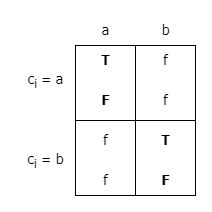
\includegraphics[width=7cm]{ACC-clauses-truth-table}
\vspace{0.1em}
\برچسب{شکل: جدول درستی برای پوشش گزاره}
\پایان{شکل}


\مهم{پوشش گزاره‌ی فعال محدود}

برای هر 
$p \in P$
 و هر گزاره‌ی اصلی 
$c_i\in C_p$
 ، گزاره‌های فرعی
$c_j, j \neq i$
 را طوری انتخاب کنید که 
$c_i$
 ارزش p را تعیین کند. مجموعه نیازمندی‌های آزمون برای هر
$c_i$
 دو شرط دارد: 
$c_i$
 به "درست" و 
$c_i$
 به "نادرست" مقداردهی شود. در هر دوی این حالت‌ها مقادیر انتخاب شده برای جملات فرعی 
$c_j$
 باید یکسان باشد.
 
برای مثال
 $p = a \vee (b \wedge c)$،
 را در نظر بگیرید برای اینکه a ارزش p را تعیین کند، عبارت
$ b \vee c$
 باید "درست" باشد. این را می‌توان به سه طریق به دست آورد: b "درست" و c "نادرست" باشد، b "نادرست" و c "درست" باشد، و یا b و c هر دو "درست" باشند. بنابراین، می‌توان پوشش گزاره‌ی فعال محدود را با توجه به گزاره‌ی a را به کمک جدول زیر مشخص کرد. 
 
در جدول درستی زیر 6 حالتی را که گزاره‌ی a تعیین‌کننده‎ی ارزش مسند p است را آورده‎ایم طبق تعریف پوشش گزاره‌ی فعال محدود، میتوان این پوشش را با توجه به بند a این‌گونه ارضا کرد. ردیف 2 را می‌توان با ردیف 6، ردیف 3 با ردیف 7، یا ردیف 1 با ردیف 5 جفت کرد. بنابراین، تنها سه روش می‌توانند پوشش گزاره‌ی فعال محدود را برآورده کنند.


\شروع{شکل}[h]
\raggedright
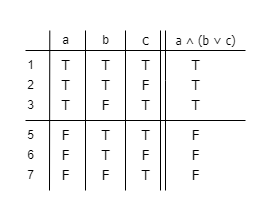
\includegraphics[width=7cm]{RACC-clauses-truth-table}
\vspace{0.1em}
\برچسب{شکل: جدول درستی برای پوشش گزاره}
\پایان{شکل}



\مهم{آزمون جهش}

در همه‌ی برنامه‌ها می‌گوییم رشته‌های ورودی اگر به زبانی باشد که یک دستور زبان\پاورقی{grammer} آن را مشخص کرده است معتبر است و در غیر این صورت نامعتبر است. به عنوان مثال، کاملاً معمول است که از یک برنامه انتظار داشته باشیم ورودی‌های نادرست را رد کند. و این ویژگی باید صراحتا آزمون شود، زیرا برای توسعه‌دهندگان آسان است که آن را فراموش کنند یا اشتباه کنند. بنابراین، تولید رشته‌های نامعتبر از دستور زبان اغلب برای ورودی آزمون‌ها مفید است. همچنین در آزمون، استفاده از رشته‌هایی که معتبر هستند اما مشتق متفاوتی از یک رشته‌ی از قبل موجود هستند، مفید است. هر دو نوع این رشته‌ها جهش‌یافته نامیده می‌شوند. تولید رشته‌های ورودی نامعتبر را می‌توان با جهش\پاورقی{mutation} دستور زبان، سپس تولید رشته‌\پاورقی{string}ها، یا با جهش مقادیر در طول یک مشتق انجام داد.

جهش همیشه بر اساس مجموعه ای از "عملگرهای جهش" است که با توجه به یک رشته‌ی "پایه" تعریف می‌شوند. رشته‎ی پایه هر رشته‌ای در گرامر می‌تواند باشد و عملگر جهش قاعده‌ای است که تغییرات نحوی رشته‌های تولید شده از یک دستور زبان را مشخص می‌‌کند. همچنین یک جهش‌یافته نیز نتیجه‌ی اعمال یک  عملگر جهش است. عملگرهای جهش معمولاً برای رشته‌های‌پایه اعمال می‌شوند، اما می‌توانند در دستور زبان یا به صورت پویا در طول اشتقاق نیز اعمال شوند\مرجع{testingbook}.

نمونه ی این عملگرها جایگزینی عملگرهای ریاضی یا رابطه‌ای، تغییر شرط شاخه\پاورقی{branch condition} و یا حذف یک عبارت\پاورقی{expression} است. نمونه ای از جهش یافته‌ها برای یک قطعه کد در ~\رجوع{جدول: جهش‎یافته‌های نمونه} آمده است.

\شروع{لوح}[t]
\وسط‌چین
\شرح{جهش‎یافته‌های نمونه} 

\شروع{جدول}{|p{0.3\linewidth} | p{0.3\linewidth} | p{0.1\linewidth}|}

\خط‌پر
  \toprule
مسند شرطی اصلی & نمونه مسند جهش‌یافته &  عملگر جهش   \\
  \midrule
 $ a < b $ &$ a \geq b $ &  ROR \\
 $ (a > b) \,\&\&\, (a > c) $ & $ (a > b) \,||\, (a > c)$ & COR  \\ 
 \خط‌پر
\پایان{جدول}
\برچسب{جدول: جهش‎یافته‌های نمونه} 
\پایان{لوح}


تحلیل جهش آزمون در موارد زیر کاربرد دارد:
\شروع {فقرات}
\فقره ارزیابی مجموعه آزمون
\فقره انتخاب مجموعه آزمون
\فقره کمینه سازی مجموعه آزمون
\فقره تولید مجموعه‌ آزمون
\فقره مکان‌یابی خطا
\فقره پیش‌بینی خطا
\پایان {فقرات}


آزمون جهش شناخته شده‌ترین روش آزمون با استفاده از تزریق خطا است؛ آزمون جهش همچنین به طور گسترده برای ارزیابی عملکرد و بهبود مجموعه‌ای از موارد آزمون به کار گرفته می‌شود \مرجع{silva2017}. آزمون جهش همچنین معمولاً به عنوان راهی برای ارزیابی کفایت مجموعه‌های آزمایشی است.این معیار با تولید یک مجموعه آزمون، نشان می‌دهد اشتباهات درج شده در جهش‌یافته‌ها در برنامه‌ی اصلی وجود ندارد، و با این کار قابلیت اطمینان برنامه را افزایش می‌دهد. برای اعمال این معیار ابتدا برنامه اصلی با مجموعه موارد آزمون اولیه اجرا می‌شود. سپس جهش یافته‌ها با همان مجموعه موارد آزمون تولید و اجرا می‌شوند. آنهایی که رفتاری متفاوت از برنامه‌‌ی اصلی دارند کشته‌شده در نظر گرفته می‌شوند و دیگر در آزمون استفاده نمی‌شوند. مجموعه‌ای از جهش یافته‌های زنده مورد تجزیه و تحلیل قرار گرفته و جهش یافته‌های هم‌ارز شناسایی می‌‌شوند. یک جهش زمانی هم‌ارز در نظر گرفته می‌شود که، برای همه موارد آزمون، دقیقاً همان رفتار برنامه‌ی تحت آزمون را نشان دهد. در نهایت، موارد آزمون جدید برای کشتن جهش یافته‌های زنده ایجاد می‌شود. علیرغم مزایای آزمایش جهش از نظر اثربخشی، برخی مشکلات مانند تعداد زیاد جهش تولید‌شده، هزینه محاسباتی مورد نیاز برای اجرای آنها و تلاش زیاد لازم برای شناسایی جهش‌یافته‌های معادل مطرح می‌شود\مرجع{roman2021}.









